% !TEX root = ../Seminararbeit-Data_Mining_Frameworks.tex
%


% =============================================================================
%
% Vorsstellung der Software
%
% =============================================================================
\chapter{Vorstellung der Software}
\label{sec:software}

\section{Rapidminer Studio}
\label{sec:software:rm}

Bei RapidMiner handelt es sich um eine „Open Source Data Science Platform“,
welche vom gleichnamigen Unternehmen unter der AGPL 3.0 Lizenz vertrieben wird.
Der Quellcode ist offen und kann auf Github gefunden werden. Neben dem im
Folgenden näher untersuchten „RapidMiner Studio“ bietet die Plattform noch die
Produkte „RapidMiner Server“ zur Automatisierung von Prozessen und „RapidMiner
Radoop“ welches es erlaubt Berechnungen in einer Hadoop Umgebung auf einem
Cluster auszuführen. Für kleinere Datensätze mit bis zu 10.000 Einträgen steht
eine kostenlose „Education Version“ zur Verfügung. Außerdem bietet der
Hersteller die Software für sämtliche Plattformen (Windows, MacOS, Linux) an. \\
Das Tool „RapidMiner Studio“ bietet die Möglichkeit einen
Datenverarbeitungsprozess mithilfe einer eingängigen Oberfläche zu erstellen.
Dafür muss die Software zunächst (auf einer der oben genannten Plattformen)
installiert werden.

\begin{figure}[htb]
	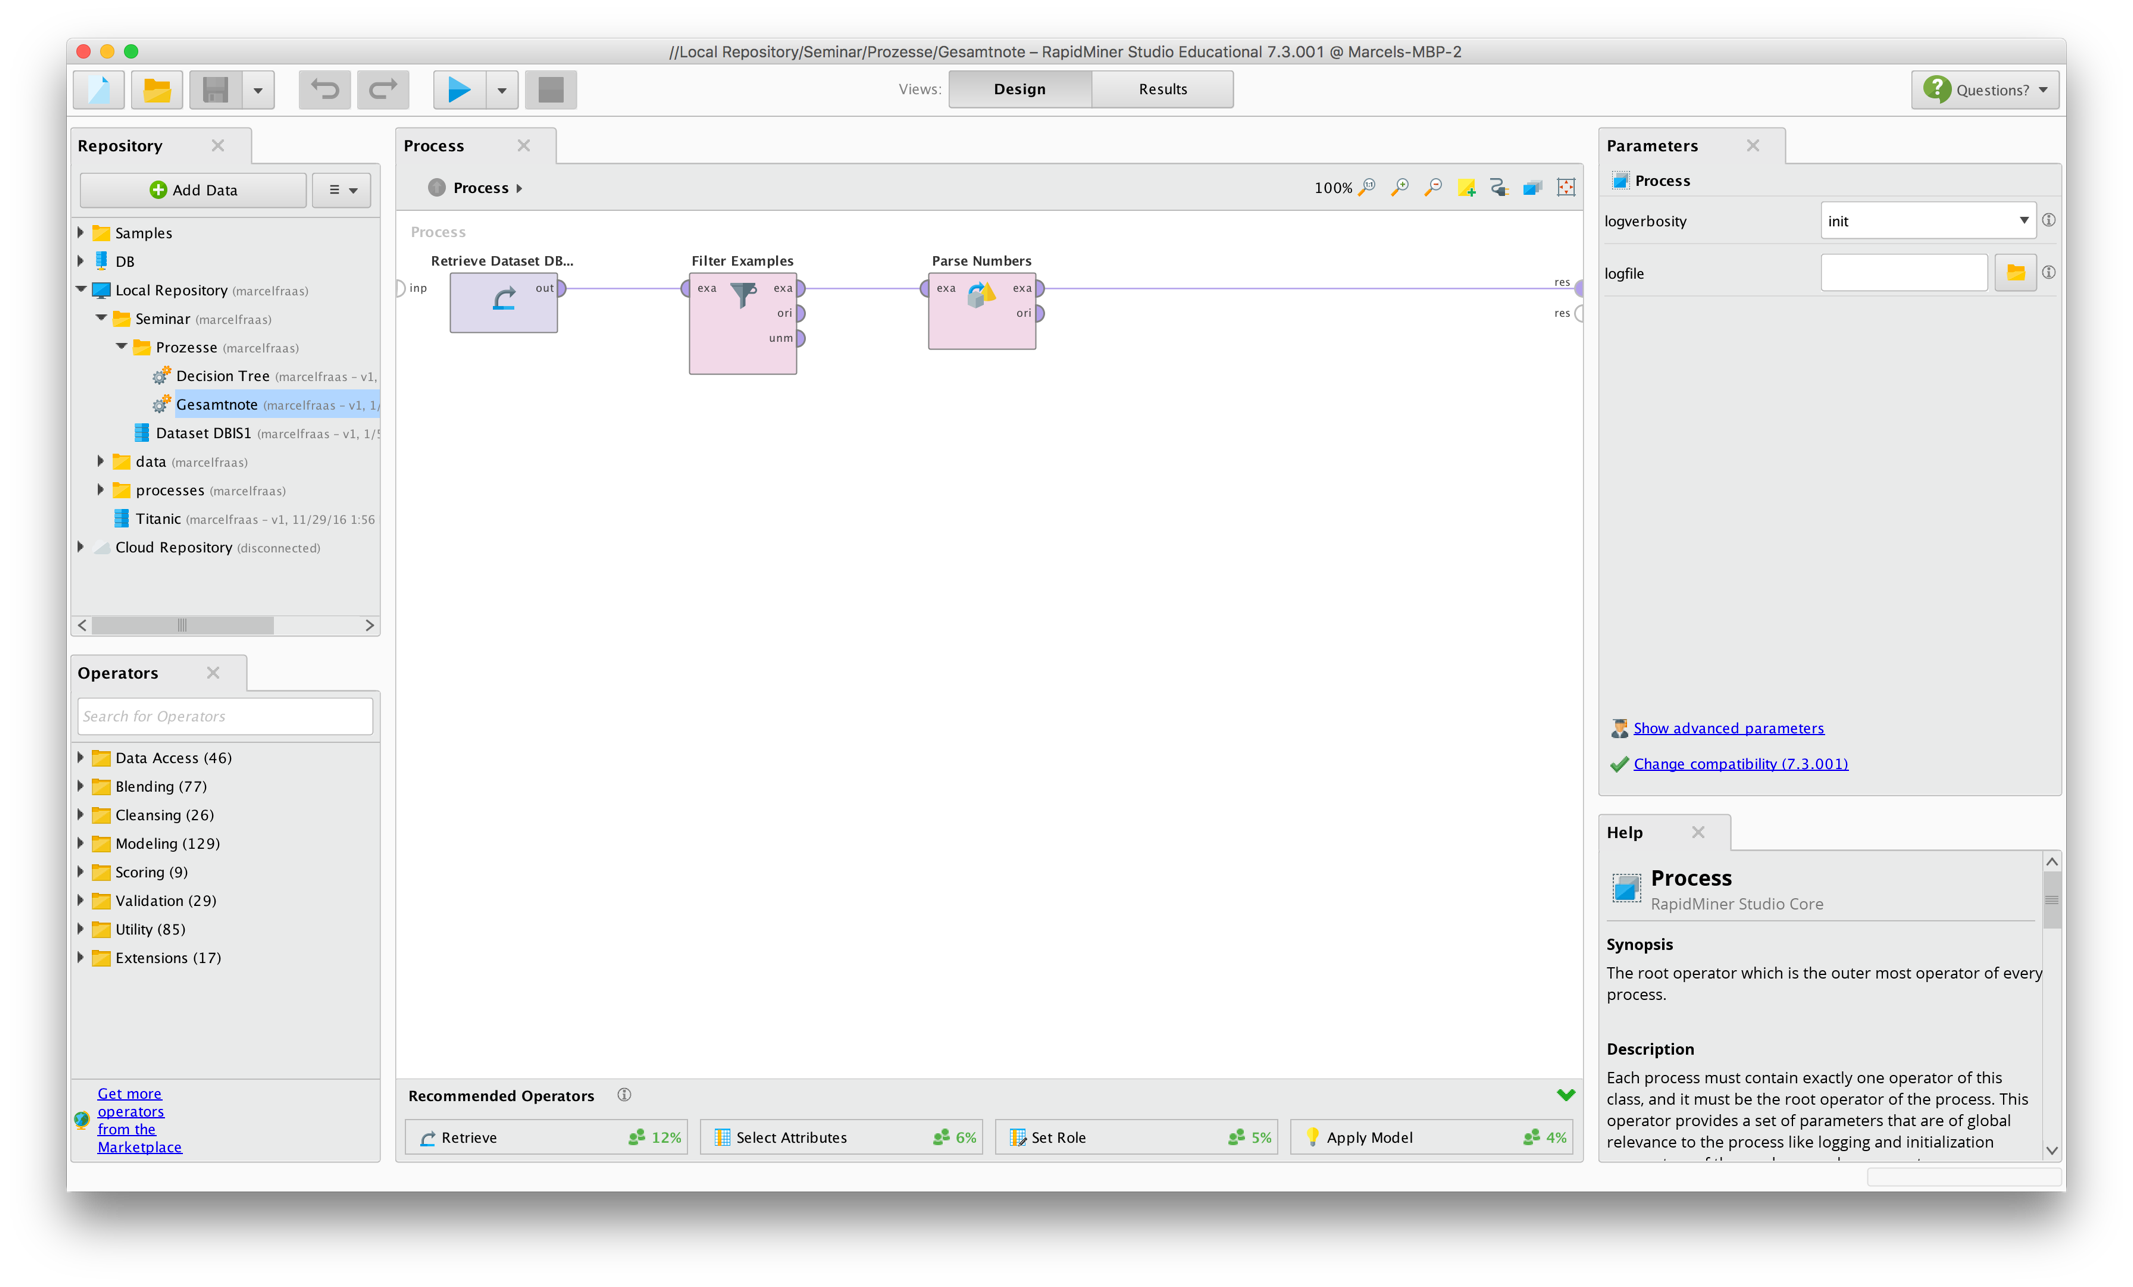
\includegraphics[width=\textwidth]{gfx/rm1.png}
	\caption{Die RapidMiner Design View}
	\label{fig:software:rm:des}
\end{figure}

Die Oberfläche bietet ein Intuitives User Interface, welches die Einarbeitung
sehr vereinfacht. Im Abschnitt links oben befindet sich das sog. „Repository“.
Hier befinden sich die konfigurierten Datenquellen, welche bspw. in Form von
Excel-, Access-, SAS oder SPSS Dateien vorliegen können. Alternativ können auch
direkt SQL Datenbanken, wie MySQL, Microsoft SQL Server, Oracle, PostgreSQL
u.a., angebunden werden. \\
Darunter befindet sich die Ordnerstruktur der „Operators“. Von hier können die
zahlreichen Operatoren per Drag and Drop in den Hauptbereich der Design-Ansicht,
dem sog. „Process“ gezogen werden. \\
In der Prozessübersicht können Operatoren und Repositories angeordnet und
miteinander verknüpft werden. \\
Auf der rechten Seite befinden sich, neben der Hilfe, noch eine Übersicht über
die Parameter des aktuell ausgewählten Operators. \\
Zu guter Letzt bietet RapidMiner Studio noch eine zusätzliche Hilfsfunktion,
die sog. „Recommended Operators“. Hier werden mit Hilfe von statistischen
Auswertungen die am wahrscheinlichsten, zum aktuellen Prozess passenden,
nächsten Operatoren angezeigt. Dies erleichtert den Einstieg in die Software ungemein.

\begin{figure}[htb]
	%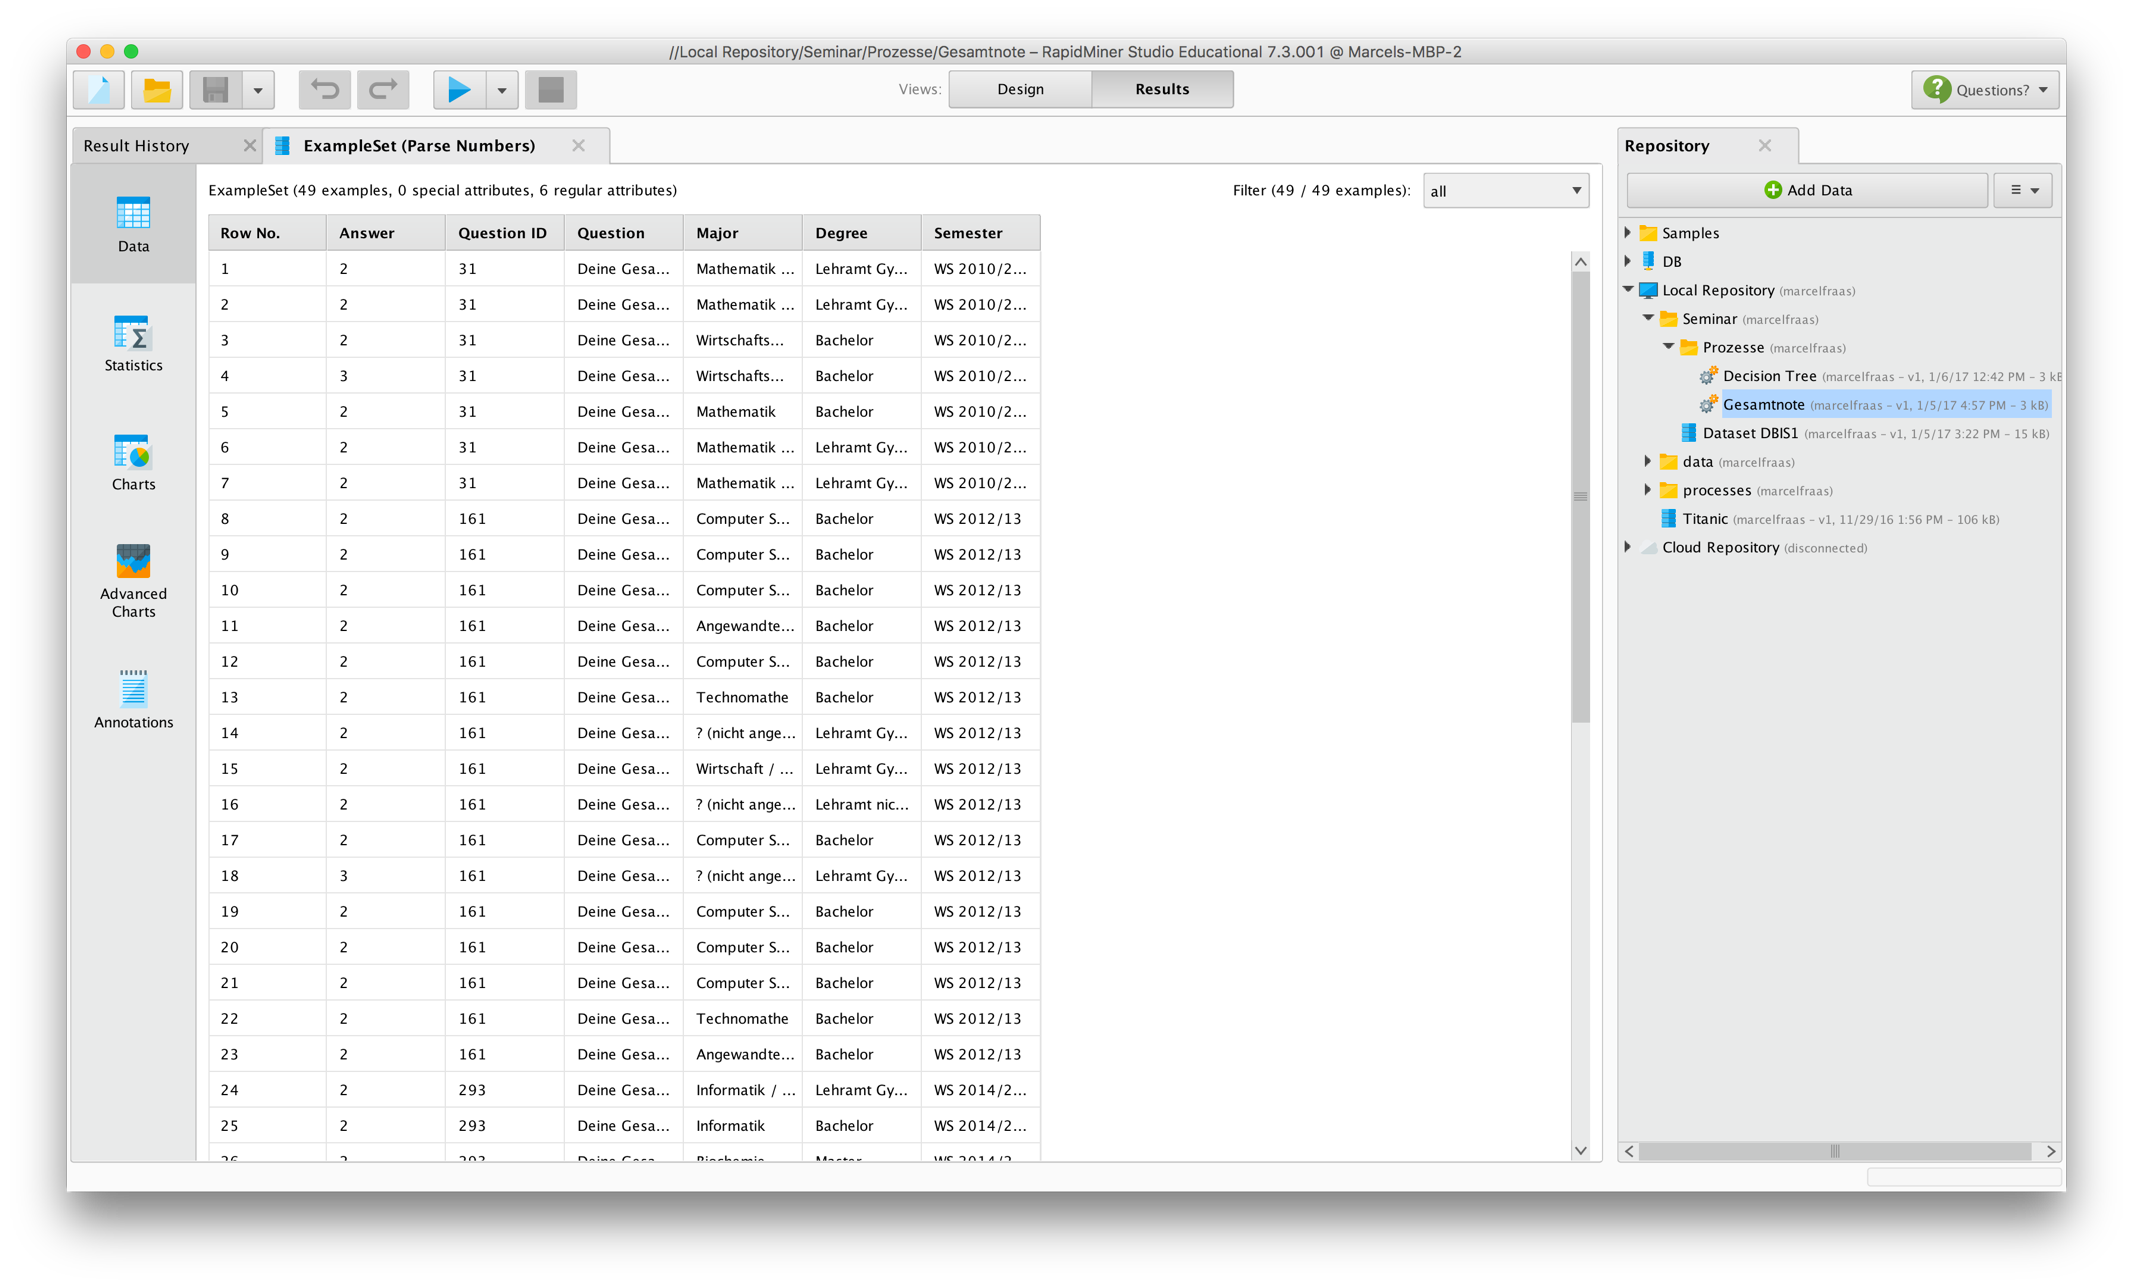
\includegraphics[width=\textwidth]{gfx/rm2.png}
  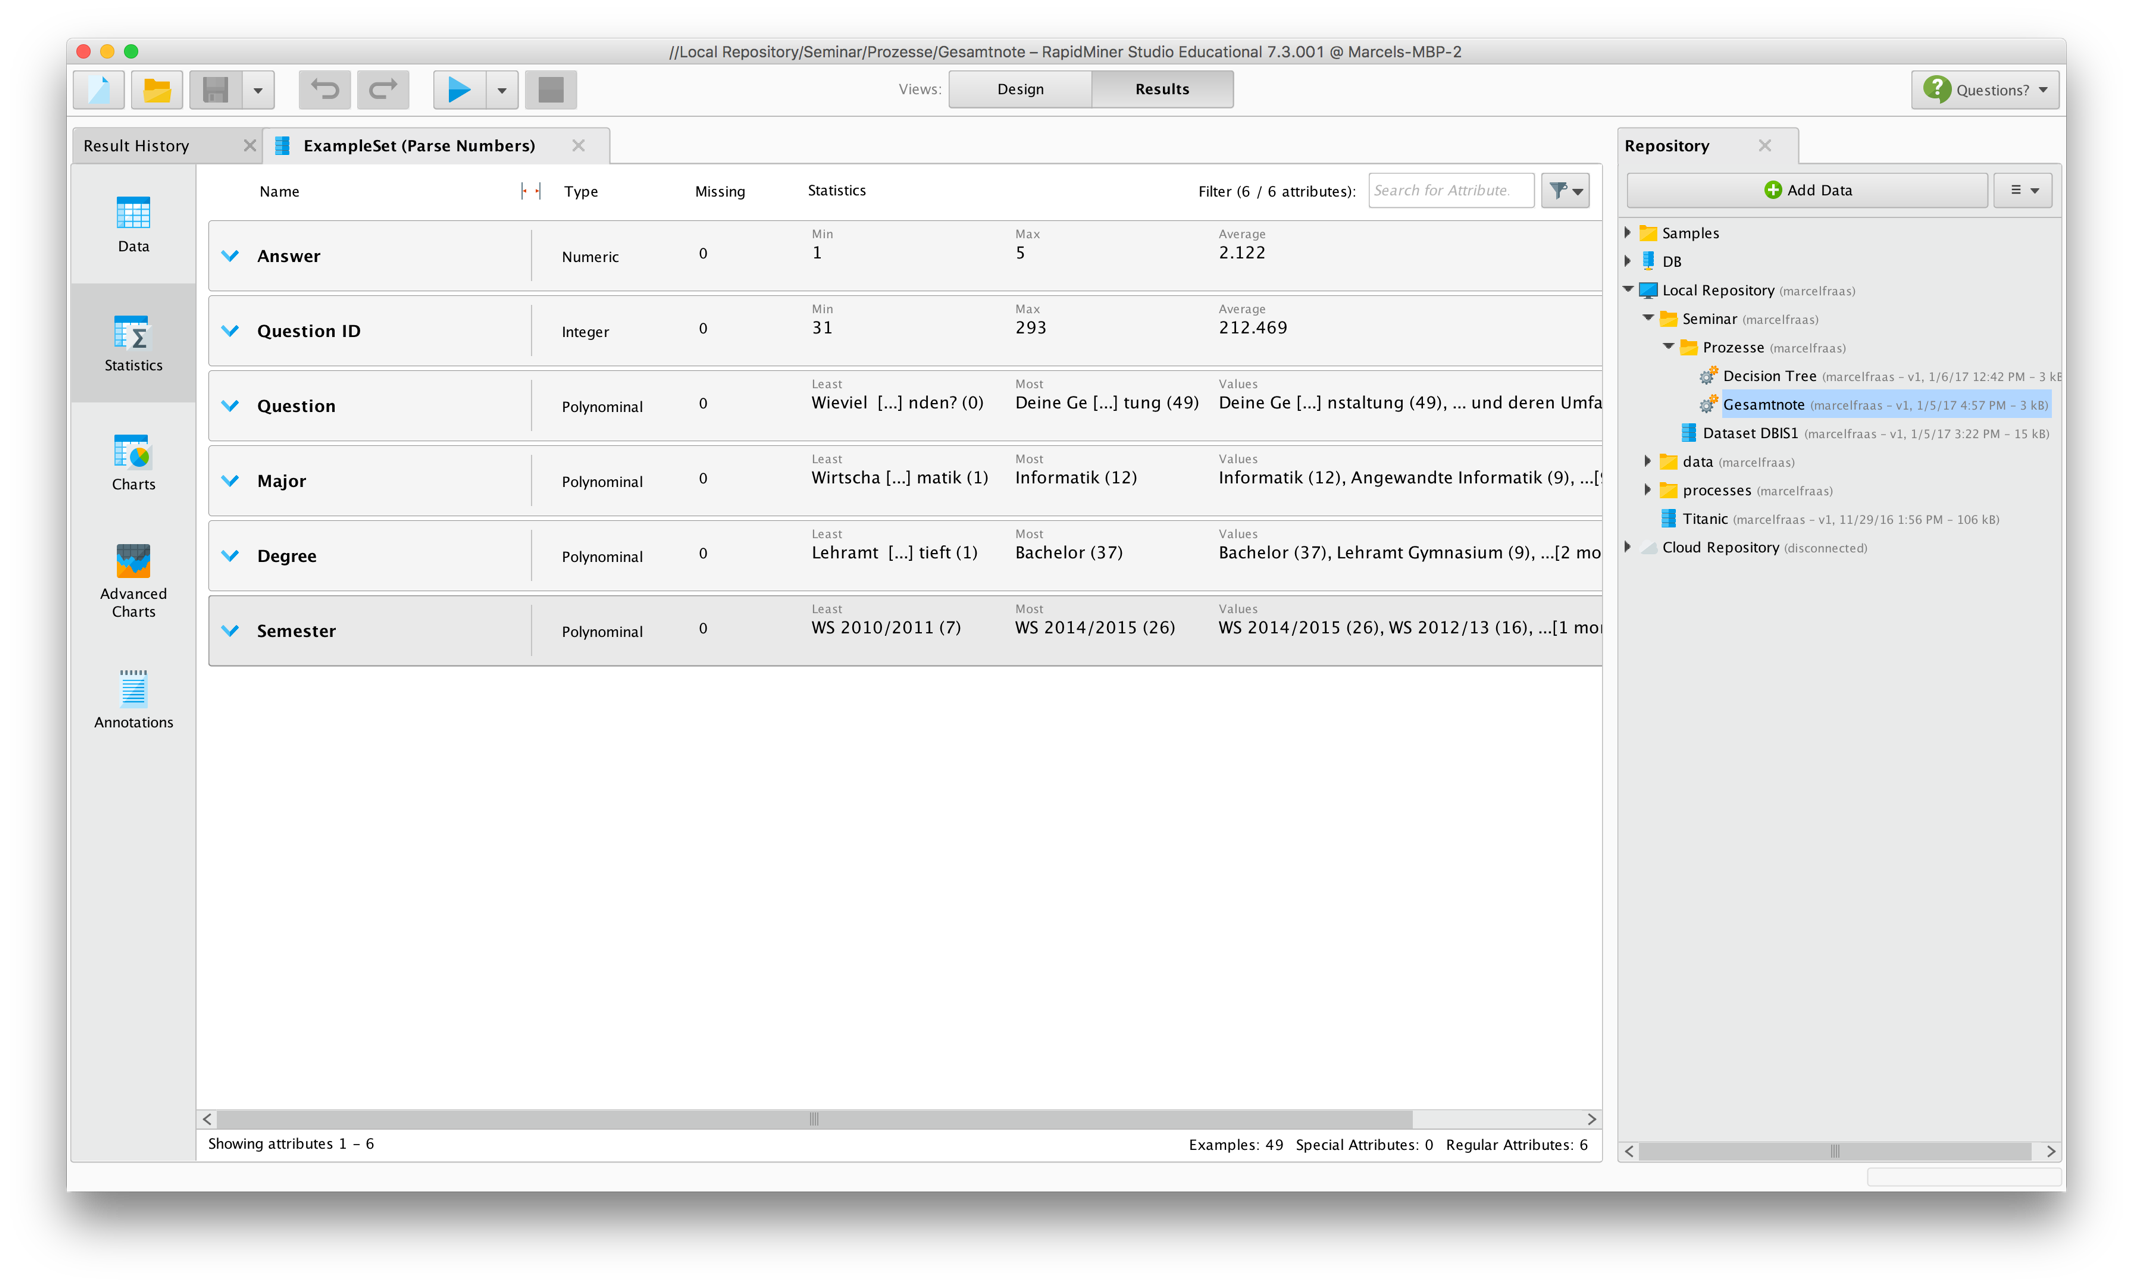
\includegraphics[width=\textwidth]{gfx/rm3.png}
	\caption{Die RapidMiner Result View}
	\label{fig:software:rm:res}
\end{figure}

Führt man einen Prozess aus, bzw. wählt man manuell in der Menüleiste den Reiter
„Results“ bekommt man das Ergebnis entweder in roh Form, also als Tabelle, in
einer statistischen Übersicht oder als Graph bzw. Diagramm.


Generell ist die Einarbeitung in RapidMiner Studio, gerade auch wegen den
detaillierten Hilfsfunktionen, sehr eingängig und führt schnell zu Ergebnissen.

\pagebreak

\section{Microsoft Azure Machine Learning Studio}
\label{sec:software:msa}

Das „Microsoft Azure Machine Learning Studio“ ist, wie der Name bereits verrät,
teil der Microsoft Cloud Umgebung Azure. Folglich ist das Tool eine Webanwendung,
welche per Browser gestartet werden kann.  Für den Einstieg benötigt man
lediglich einen Microsoft Azure Account, welchen man kostenlos erstellen kann.
Damit hat man dann vollen Zugriff auf alle Funktionen des Machine Learning
Studios. Einschränkungen des kostenlosen Accounts gibt es hier nur bezüglich
der Rechenzeit und den weiteren Services der Azure Umgebung (APIs etc.). \\
Neben dem Machine Learning Studio bietet die Microsoft Cloud eine Vielzahl an
Services und Ressourcen, wie virtualisierte Server, Hosting von Webanwendungen
und APIs sowie Datenbanken. Durch den „Platform as a Service“ Aspekt, wird eine
extrem einfache Kollaboration und schnelles Deployment ohne eigenen
Administrationsaufwand gewährleistet.

\begin{figure}[htb]
	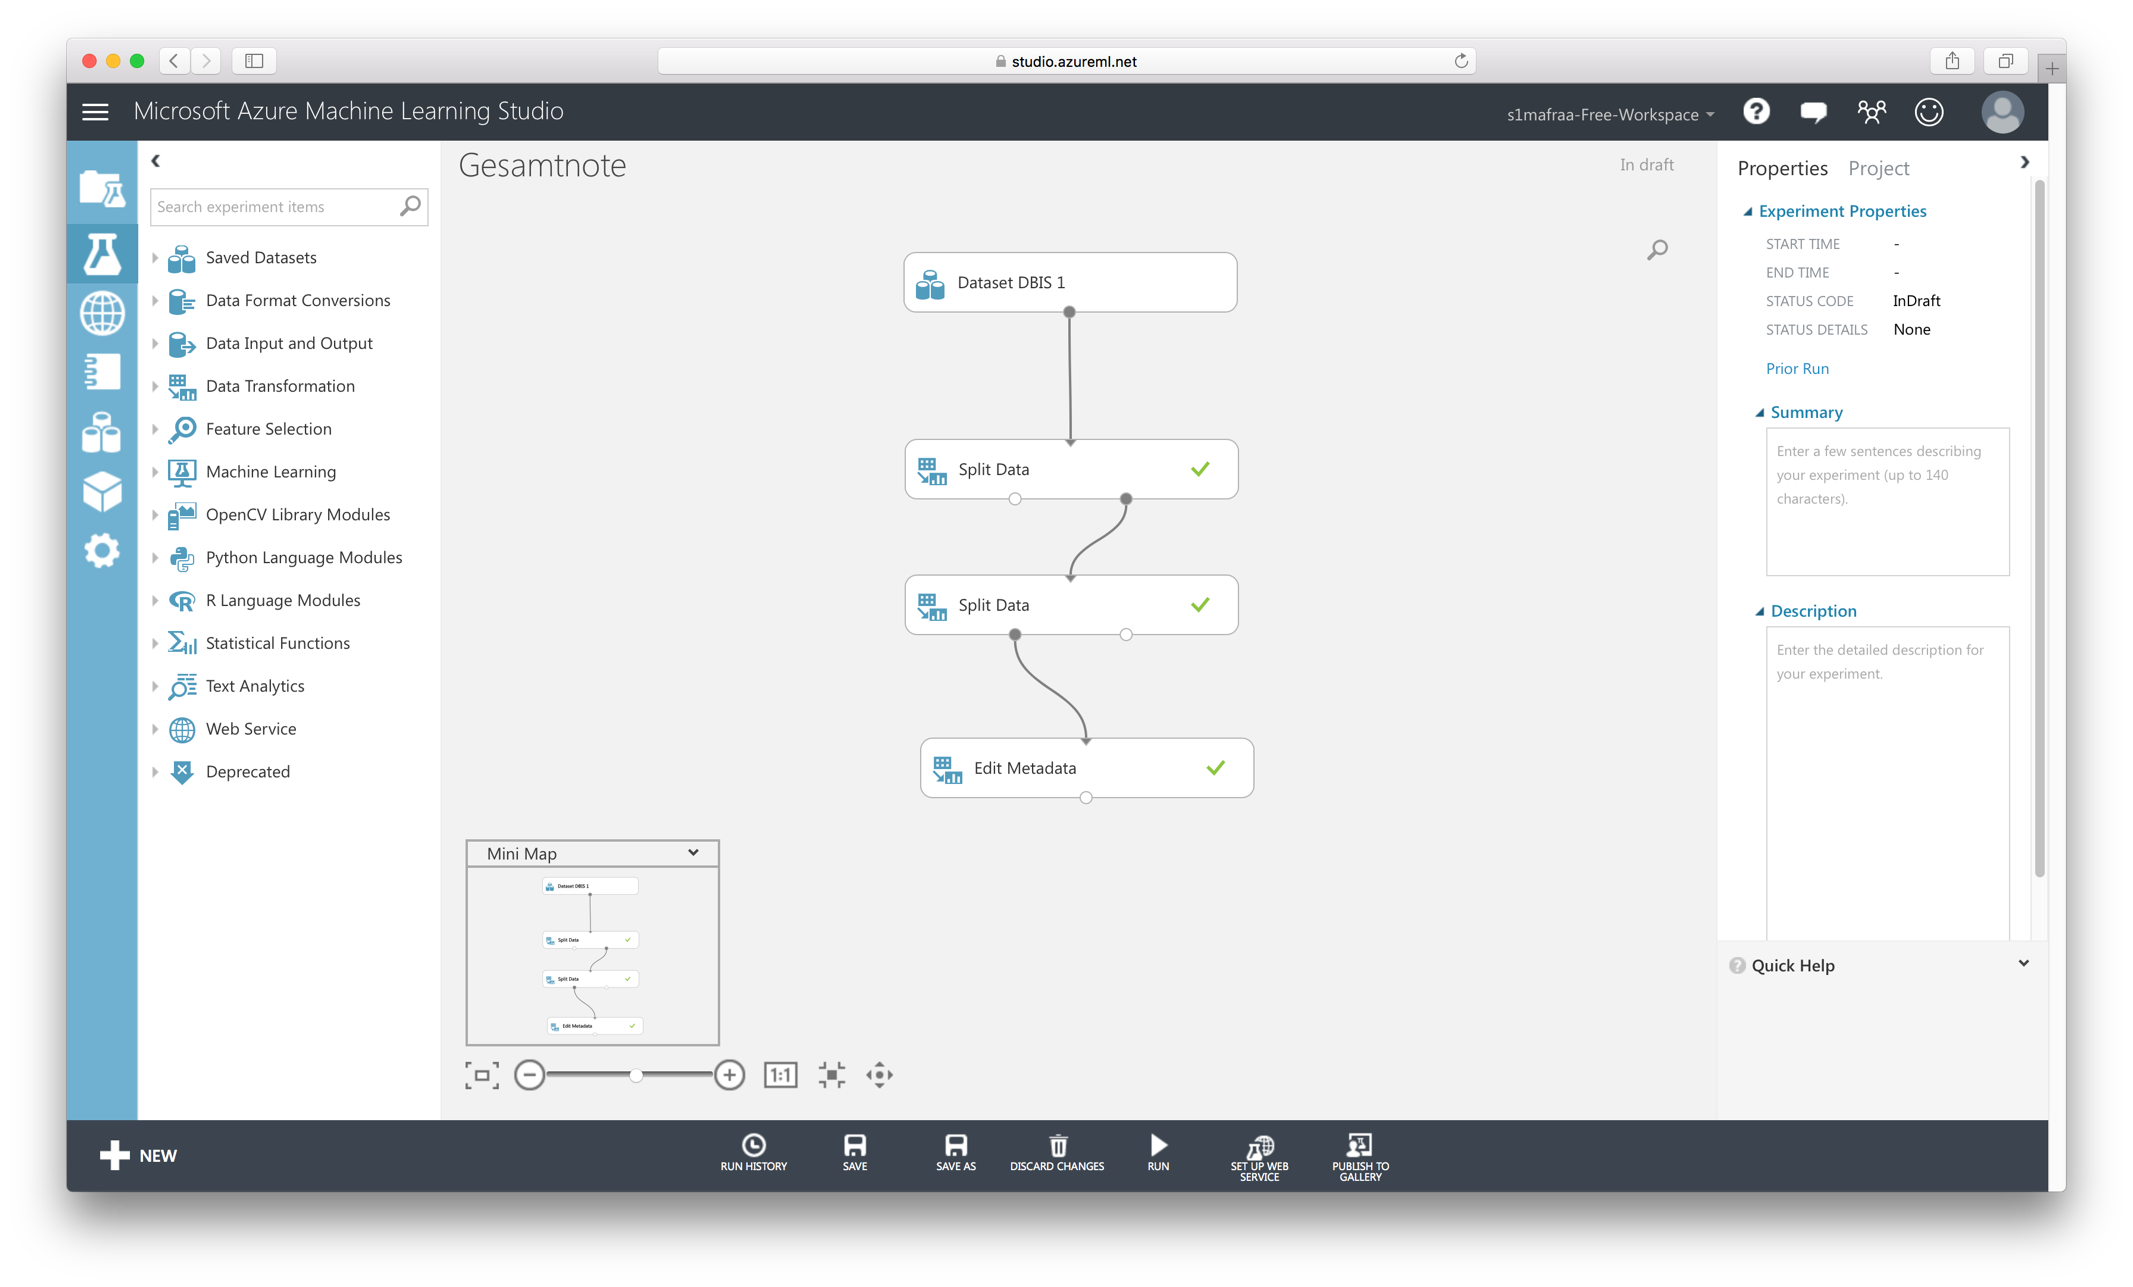
\includegraphics[width=\textwidth]{gfx/ml1.png}
	\caption{Ein Expriment im MSA Machine Learning Studio}
	\label{fig:software:ml:des}
\end{figure}

Nach dem starten der Webanwendung kann der Anwender direkt damit beginnen ein
neues Experiment anzulegen. Die Oberfläche ist ähnlich dem RapidMiner User
Interface aufgebaut. Auf der linken Seite befinden sich die Datenquellen und
die Operatoren. Unterstützt werden von Microsoft u.a. die Excel-, CSV-, ARFF-,
sowie Plain Text und RObject Dateiformate. Außerdem können natürlich ebenfalls
Daten aus einer SQL Datenbank, wie beispielsweise einer Microsoft SQL
Serverinstanz aus der Azure Cloud, geladen werden. \\
Auch hier können die Operatoren per Drag and Drop in die Arbeitsfläche gezogen
werden und mit den Parametern am rechten Rand konfiguriert werden.

\begin{figure}[htb]
	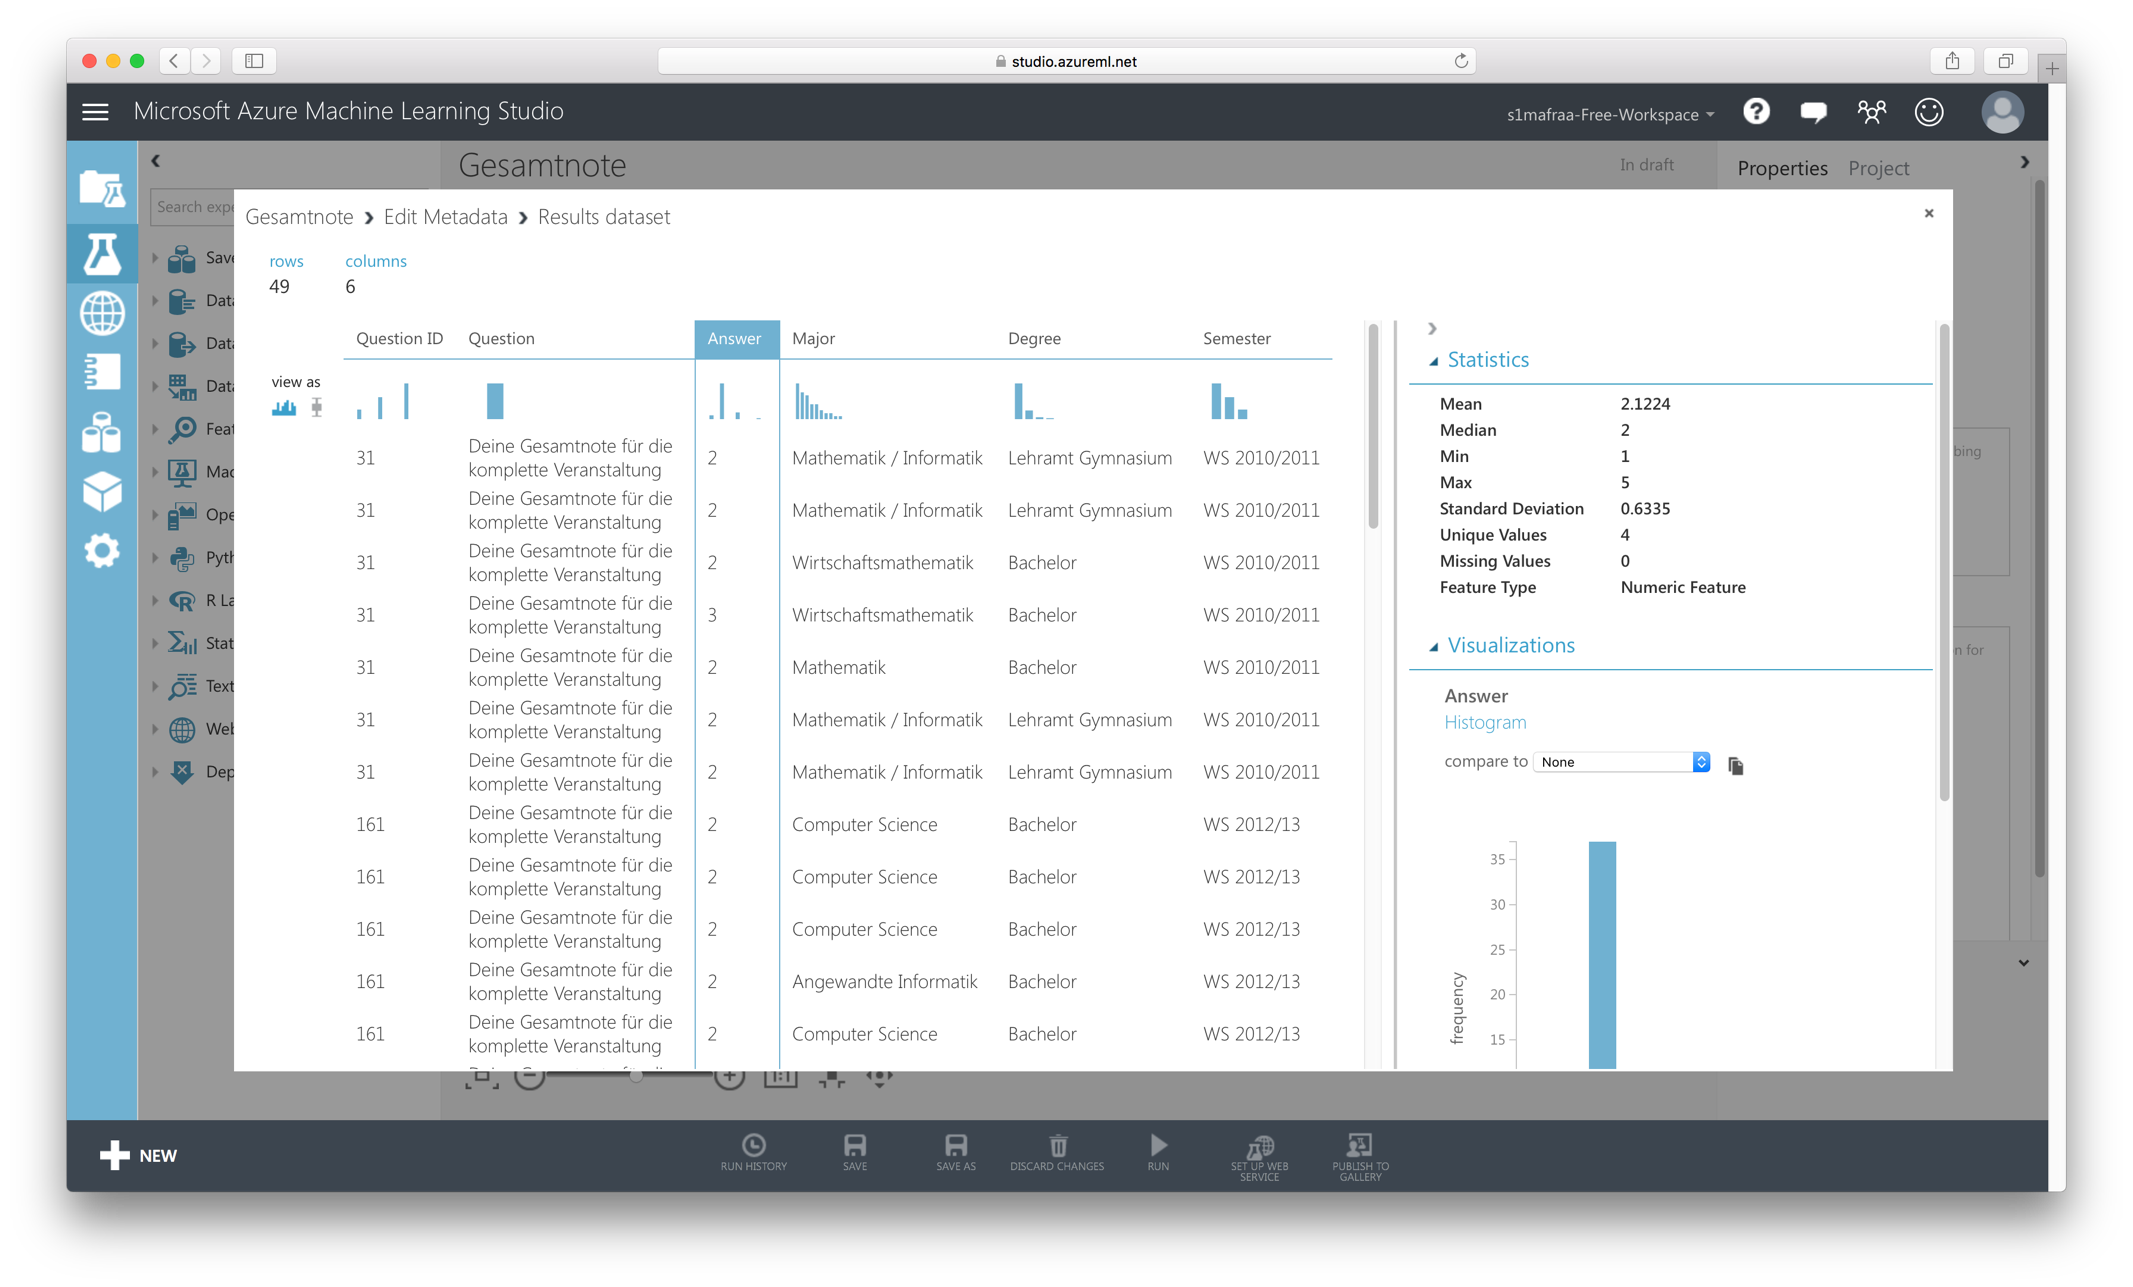
\includegraphics[width=\textwidth]{gfx/ml2.png}
	\caption{Das Ergebnis eines Expriments im MSA Machine Learning Studio}
	\label{fig:software:ml:res}
\end{figure}

Die Visualisierung des Ergebnisses ist im Machine Learning Studio abhängig vom
jeweiligen Experiment. In diesem Fall wird dieses als Tabelle mit einigen
Statistiken und Diagrammen dargestellt.


Aufgrund der Tatsache, dass es sich beim Microsoft Azure Machine Learning Studio
um eine Webanwendung handelt, müssen ein paar Abstriche in Sachen Bedienbarkeit
gemacht werden. Dafür ist die Kollaboration mit Anderen und die Einbindung in
Webservices erheblich vereinfacht, was besonders zum Tragen kommt, wenn man
bereits eine gewisse Infrastruktur innerhalb der Azure Cloud besitzt.
